%%% - - -   UNCLASSIFIED   - - - %%%

\documentclass[11pt, letterpaper]{article}

\newcommand{\thisdocument}{MILSTD}

\usepackage{format/NGICStyle}        % does everything
\usepackage{format/DurandalBib}      % contains bibliography info
\usepackage{format/NGICGlossary}     % contains glossary info
\usepackage{values/T150ModelValues}   % sets model values

%%% document settings

%% document paths
\graphicspath{{images}}
\newcommand\csvpath{csv}

\makeatletter
\def\input@path{{content}}
\makeatother

% header and footer
\chead{\documentlabel}
\cfoot{\documentlabel\ \\ \thepage}

% suppress guidance notes
\presetkeys{todonotes}{disable}{}

%%% document start
\begin{document}

\pagenumbering{roman}

\InDevelopmentfalse

\ifInDevelopment
	\draft
	\linenumbers
	\colorlet{ModelValueColor}{blue!50!cyan}
\fi

%% ============================================================
%%  FRONT MATTER -- Title Page
%% ============================================================

\begin{center}
    \vspace*{0.3in}
    \Huge\textbf{\LARGE\unclass Accreditation Plan\\}
    \vspace*{0.15in}
    \Large\textbf{\unclass T-150/TRV-150 Heavy-Lift UAS\\AFSIM Simulation Model v2.0\\}
    \normalsize\textbf{\unclass AFSIM Project 005\\}
    \vspace*{0.3in}
    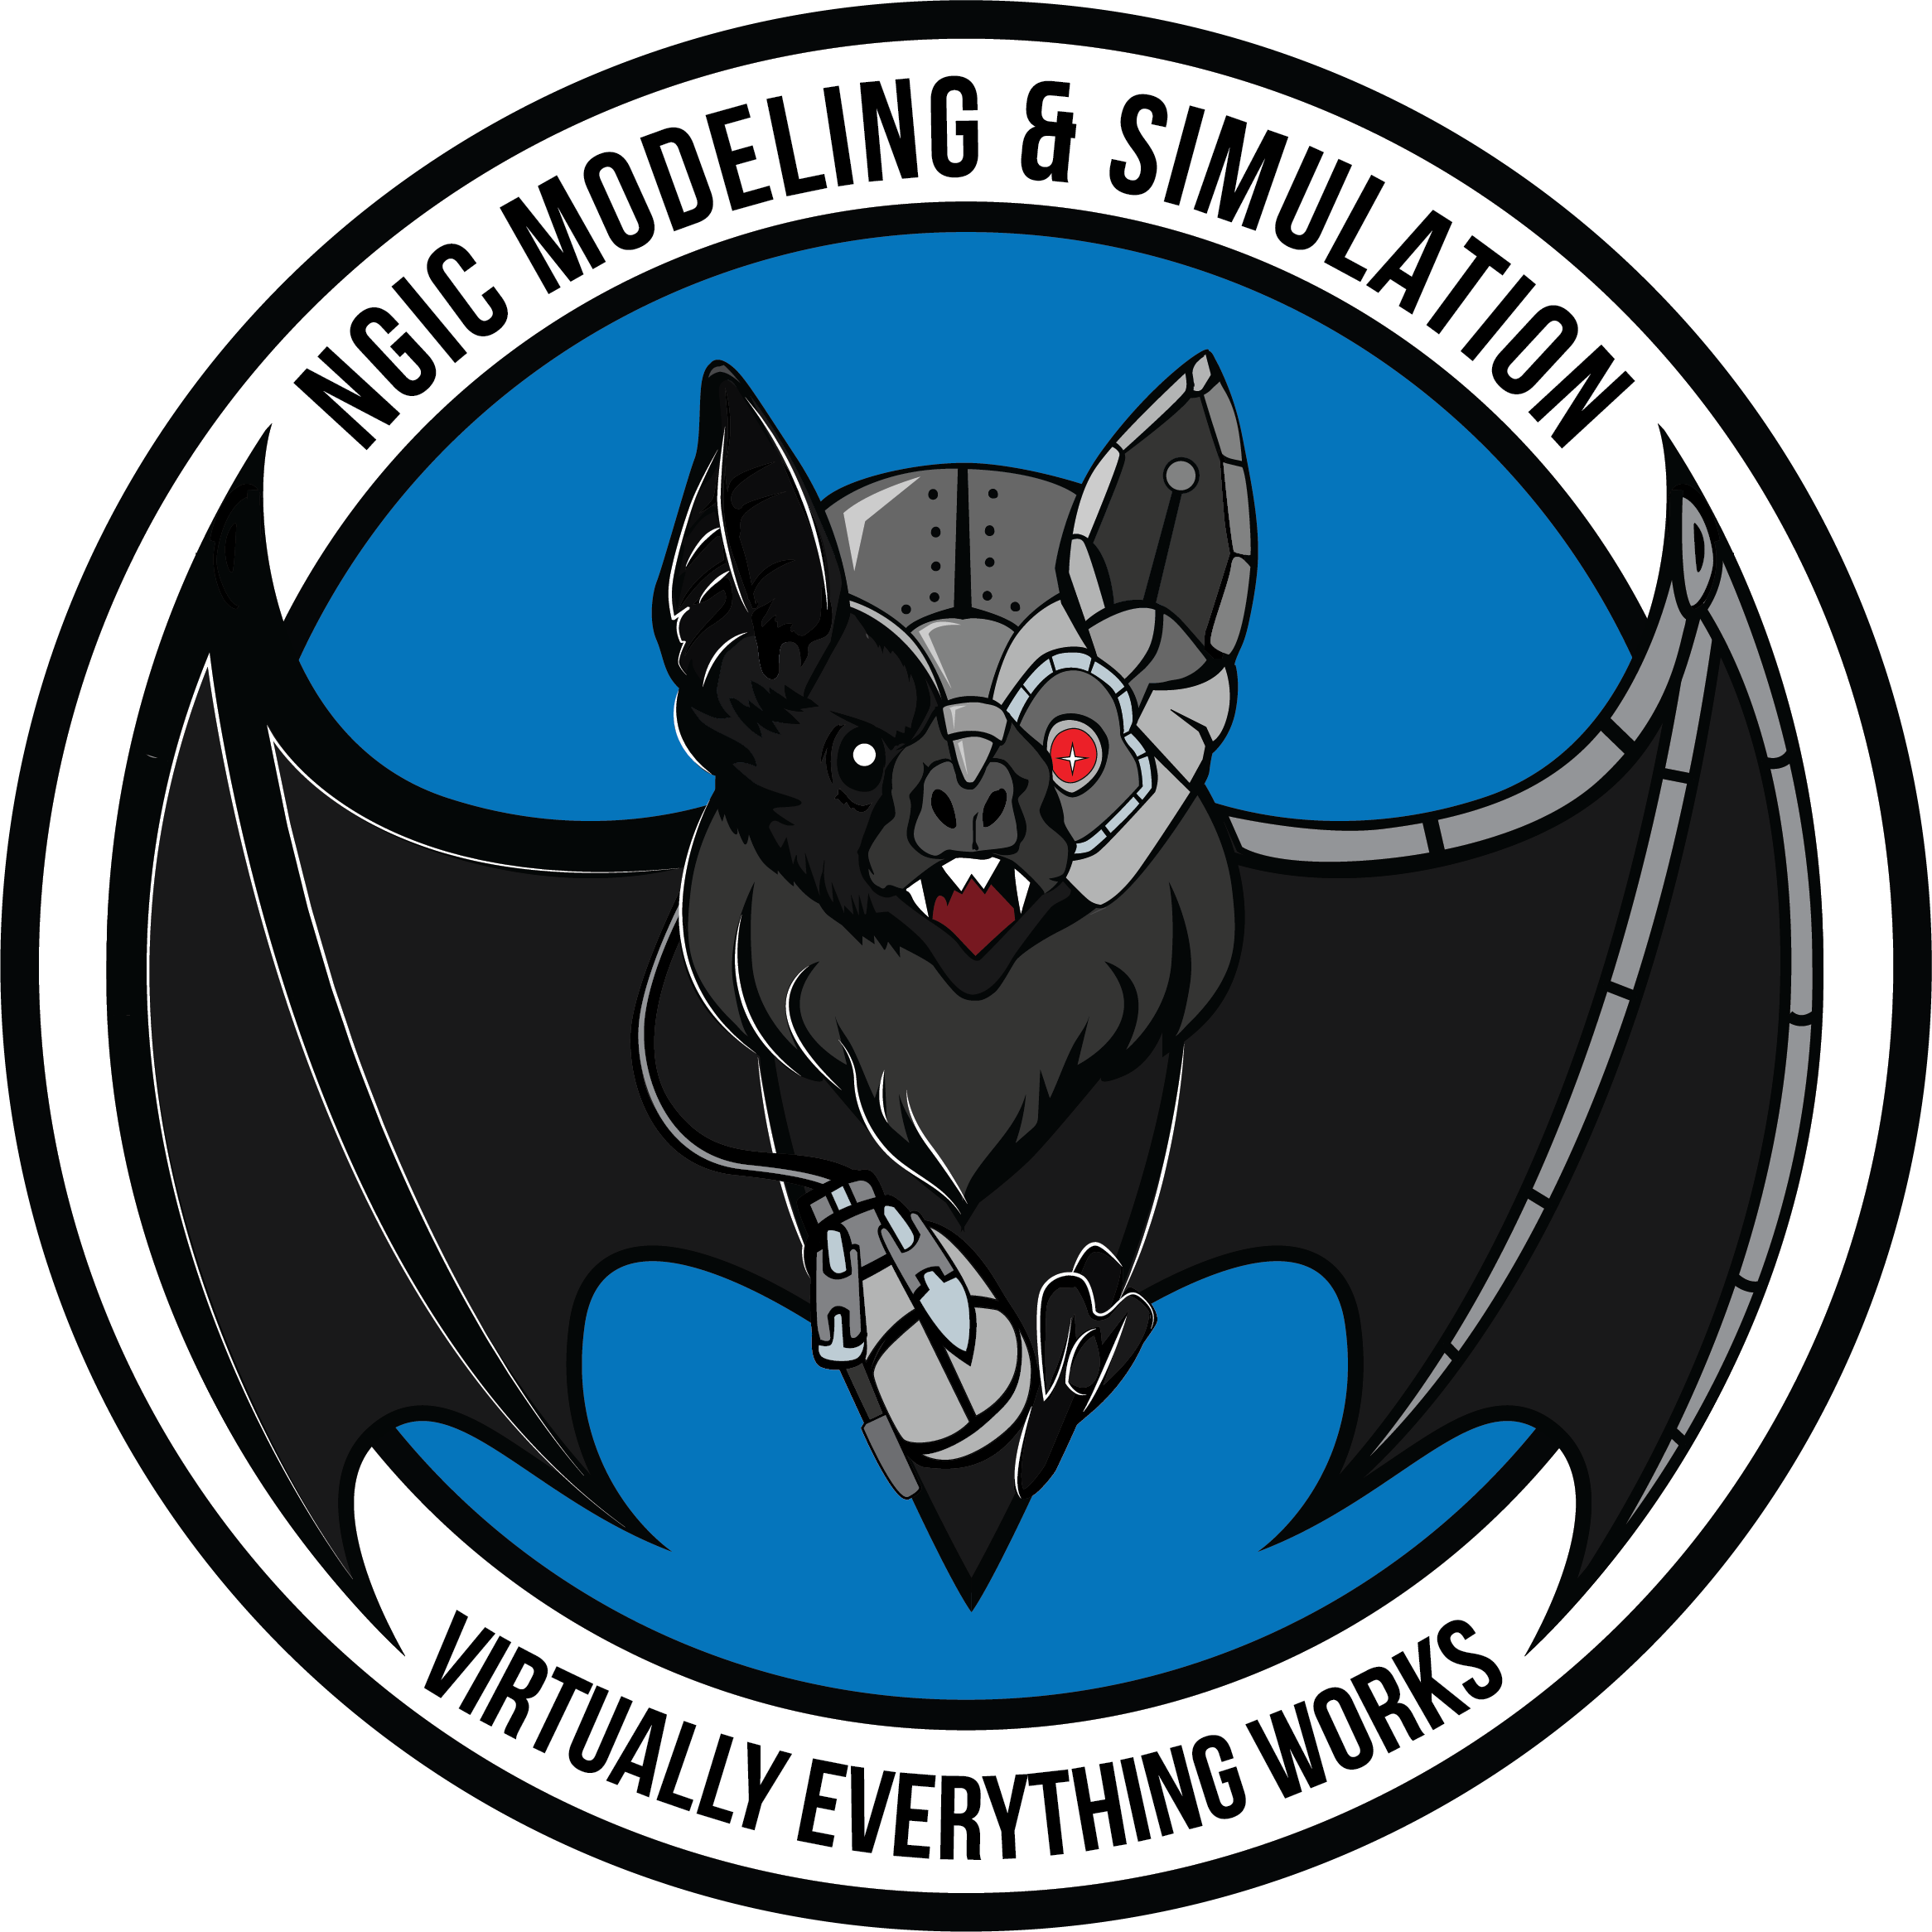
\includegraphics[width=4in]{images/ngic}

    \vspace*{0.1in}
    \Large
    \textbf{Version: 1.0 \\
    Date: March 5, 2026 \\
    Classification: UNCLASSIFIED \\}
\end{center}

\vfill

\tableTwoNow{\unclasslabel}{\unclass Document Information}{accplan-docinfo}{l,2.5in}{l,3.5in}
{
    Field & Value \\
    Document Version & 1.0 \\
    Date & March 5, 2026 \\
    Classification & UNCLASSIFIED \\
    Sponsoring Organization & [PLACEHOLDER - Organization Name] \\
    Accreditation Authority & [PLACEHOLDER - Accreditation Authority Name/Title] \\
    Program Manager & [PLACEHOLDER - Name/Title] \\
    Document Preparer & [PLACEHOLDER - Organization/Contract] \\
    Distribution Statement & [PLACEHOLDER - Distribution Statement] \\
    M\&S Name and Version & T-150 UAS AFSIM Plugin Suite v2.0 \\
}

\pagebreak

%% Record of Changes
\begin{center}
    \begin{tblr}
        {
            colspec     ={|Q[c,1in]|Q[c,1in]|Q[c,2in]|Q[2in]|},
            hline{1-Z}  ={.5pt},
            cell{1}{1}  ={c=4}{halign=l},
            cell{Z}{1}  ={c=4}{halign=r},
            row{2}      ={bg=TableBlue,fg=white,halign=c},
            cell{2-Y}{1}={halign=c},
        }
        \unclasslabel\\
        Version & Date     & Author   & Description \\
        1.0     & 2026-03-05 & {[PLACEHOLDER]}  & Initial release per MIL-STD-3022 Appendix A \\
        \unclasslabel\\
    \end{tblr}
\end{center}

\vfill
\pagebreak

%% TOC
\tableofcontents\thispagestyle{fancy}\pagebreak
\listoftables\thispagestyle{fancy}\pagebreak

% arabic numbering
\pagenumbering{arabic}
\cfoot{\classlabel\ \\ {Page \thepage\ of \pageref{LastPage}}}


%% ============================================================
%%  EXECUTIVE SUMMARY
%% ============================================================

\section{\unclass Executive Summary}

\unclass This Accreditation Plan establishes the framework and methodology for determining whether the T-150/TRV-150 Heavy-Lift UAS AFSIM Simulation Model v2.0 is acceptable for its intended use in intelligence analysis at the National Ground Intelligence Center (NGIC). The plan is prepared in accordance with MIL-STD-3022, ``Documentation of Verification, Validation, and Accreditation (VV\&A) for Models and Simulations,'' and supports the requirements of DoDI 5000.61, ``DoD Modeling and Simulation Verification, Validation, and Accreditation.''

\unclass The T-150 UAS AFSIM Plugin Suite v2.0 is a physics-based simulation model comprising five custom C++ plugins (approximately 7,736 lines of code) integrated with the Advanced Framework for Simulation, Integration, and Modeling (AFSIM). The model represents the Malloy Aeronautics T-150 (also designated TRV-150), a coaxial octocopter heavy-lift UAS with a maximum takeoff weight of 123~kg and a payload capacity of 55~kg. The model was developed to support NGIC intelligence analysis including assessment of operational performance, flight endurance, mission profiles, vulnerable flight regimes, and payload impacts on UAS capabilities.

\unclass The five plugins provide: (1) 6DOF rigid-body flight dynamics with quaternion attitude representation, (2) battery state-of-charge tracking with voltage sag modeling, (3) propulsion system modeling with thermal dynamics and ground effect, (4) Vortex Ring State detection and severity assessment, and (5) slung load pendulum dynamics. Together, these plugins deliver a high-fidelity representation of the T-150 platform within the AFSIM scenario-based analysis framework.

\unclass This plan defines the accreditation scope, identifies information needs, describes the methodology for collecting and assessing evidence, and catalogs known issues that the Accreditation Authority must consider. The model is proposed for accreditation in the domain of intelligence analysis of T-150/TRV-150 class heavy-lift UAS. The model is explicitly \textbf{not} proposed for accreditation for real-time flight control, safety-critical decision-making, acquisition milestone decisions, or live-virtual-constructive training.

\unclass Key accreditation considerations include the absence of T-150 flight test data for direct validation, a simulated flight endurance gap relative to manufacturer specifications (14.3~minutes simulated vs.\ 36~minutes manufacturer-claimed), the use of developer self-testing rather than independent V\&V, and the novel use of AI-assisted development methodology. These issues are documented in Section 5 and will require explicit disposition by the Accreditation Authority.

\pagebreak

%% ============================================================
%%  SECTION 1 -- Problem Statement
%% ============================================================

\section{\unclass Problem Statement}

\subsection{\unclass Intended Use}

\unclass The T-150 UAS AFSIM Simulation Model v2.0 is intended for use by NGIC analysts to conduct intelligence analysis of the T-150/TRV-150 class heavy-lift UAS. Specific analytical objectives include:

\begin{itemize}
    \item \unclass \textbf{Operational Performance Assessment}: Evaluate flight dynamics, speed, climb rate, descent rate, and maneuvering characteristics under various configurations and payload conditions.
    \item \unclass \textbf{Flight Endurance Analysis}: Determine battery-limited mission duration across different flight profiles (hover, cruise, mixed mission), payload weights, and environmental conditions.
    \item \unclass \textbf{Mission Profile Analysis}: Simulate representative mission profiles to assess operational utility, including cargo delivery, surveillance orbits, and ingress/egress routes.
    \item \unclass \textbf{Vulnerable Flight Regime Identification}: Identify flight conditions (e.g., steep descent at low forward speed) where the platform is susceptible to Vortex Ring State or other loss-of-control phenomena.
    \item \unclass \textbf{Payload Impact Assessment}: Quantify the effects of payload mass and configuration (internal vs.\ slung load) on flight performance, endurance, and stability.
    \item \unclass \textbf{C-UAS Assessment Support}: Provide simulation inputs for Counter-UAS analysis including observable flight characteristics, engagement window estimation, and vulnerability assessment.
    \item \unclass \textbf{CONOPS Development}: Support the development of concepts of operations for employment of T-150 class UAS in adversary force structures.
\end{itemize}

\subsection{\unclass M\&S Overview}

\unclass The T-150 UAS AFSIM Plugin Suite v2.0 consists of five custom C++ AFSIM plugins totaling approximately 7,736 lines of code. The plugins implement physics-based flight dynamics with subsystem-level modeling:

\tableFouNow{\unclasslabel}{\unclass Plugin Suite Components}{accplan-plugins}{l,1.3in}{l,1.5in}{c,0.5in}{l,2.5in}
{
    Plugin & AFSIM Type & LOC & Function \\
    rotorcraft\_6dof & WSF\_ROTORCRAFT\_6DOF\_MOVER & $\sim$4,085 & 6DOF rigid-body mover with quaternion attitude, rotor model, flight controllers \\
    t150\_battery & T150\_BATTERY\_PROCESSOR & $\sim$1,139 & Battery SOC/voltage/current tracking with voltage sag model \\
    t150\_propulsion & T150\_PROPULSION\_PROCESSOR & $\sim$1,395 & 8-motor propulsion, thermal model, ground effect, dynamic power \\
    t150\_vrs & T150\_VRS\_PROCESSOR & $\sim$697 & VRS detection, state machine, lift/control degradation factors \\
    t150\_slung\_load & T150\_SLUNG\_LOAD\_PROCESSOR & $\sim$825 & 2-DOF spherical pendulum slung load dynamics \\
}

\unclass The model operates within the AFSIM simulation framework (v2.2505), leveraging AFSIM's scenario management, event recording, and visualization capabilities. Inter-plugin communication uses the AFSIM AuxData key-value interface.

\subsection{\unclass M\&S Application}

\unclass The simulation model provides a high-fidelity UAS platform representation for scenario-based analysis within the AFSIM framework. Analysts configure scenarios using AFSIM text-based scenario files (.afsim) that define platform parameters, mission routes, environmental conditions, and output recording. The model produces time-series telemetry (position, velocity, attitude, battery state, propulsion state, VRS status, and slung load dynamics) that analysts use to assess platform capabilities and limitations.

\unclass The model supports both individual scenario execution and batch analysis across parameter sweeps (e.g., varying payload mass to determine performance degradation curves).

\subsection{\unclass Accreditation Scope}

\unclass \textbf{In Scope}: The model is proposed for accreditation for use in intelligence analysis of T-150/TRV-150 class heavy-lift UAS, including the analytical applications listed in Section 1.1.

\unclass \textbf{Out of Scope -- The model is NOT accredited for}:

\begin{itemize}
    \item \unclass Real-time flight control or hardware-in-the-loop applications
    \item \unclass Safety-critical decisions (e.g., airspace deconfliction, collision avoidance)
    \item \unclass Acquisition milestone decisions or cost-benefit analyses
    \item \unclass Live-virtual-constructive (LVC) training exercises
    \item \unclass Analysis of UAS platforms substantially different from the T-150/TRV-150 coaxial octocopter configuration without re-parameterization and re-validation
\end{itemize}

\pagebreak

%% ============================================================
%%  SECTION 2 -- M&S Requirements and Acceptability Criteria
%% ============================================================

\section{\unclass M\&S Requirements and Acceptability Criteria}

\unclass The following table maps M\&S requirements to acceptability criteria and metrics. These requirements derive from the intended use described in Section 1.1 and are traceable to the test cases documented in the V\&V Report.

\tableFivNow{\unclasslabel}{\unclass Requirements and Acceptability Criteria}{accplan-reqs}{c,0.5in}{l,1.5in}{l,1.5in}{l,1in}{l,1in}
{
    Req ID & Requirement & Acceptability Criterion & Metric & V\&V Evidence \\
    REQ-01 & Flight dynamics fidelity & Stable 6DOF physics; drift $<$ 1.0~m; velocity tracking error $<$ 1.0~m/s & No NaN/divergence; position hold drift $<$ 1.0~m & Phase 1 Tests 01--05 \\
    REQ-02 & Energy system accuracy & SOC tracking with $<$ 0.1\% cumulative error; correct voltage sag & Energy balance error $<$ 0.1\%; monotonic SOC decrease & Phase 1 Tests 06, 09 \\
    REQ-03 & VRS detection accuracy & Correct VRS state transitions at documented thresholds & VRS onset at descent rate $\geq$ 4.0~m/s with forward speed $<$ 5.0~m/s & VRS processor unit testing \\
    REQ-04 & Performance envelope fidelity & Cruise speed within 10\% of manufacturer specification & Max cruise speed 27--33~m/s; MTOW 123~kg & Phase 1 Test 04 \\
    REQ-05 & Subsystem interaction correctness & Correct AuxData communication between all plugins & All 68 AuxData keys published correctly & Integration testing \\
    REQ-06 & Ground effect modeling & Thrust augmentation near ground consistent with Cheeseman-Bennett & Ground effect factor 1.0--1.3; active below 1 rotor diameter AGL & Phase 1 Test 07 \\
    REQ-07 & Motor thermal dynamics & Realistic motor temperature response to power draw & Temperature equilibrium 60--90$^\circ$C at hover & Phase 1 Test 01 \\
    REQ-08 & Slung load dynamics & Physically correct pendulum behavior with appropriate natural frequency & Natural frequency matches $f = \frac{1}{2\pi}\sqrt{g/L}$ & Slung load unit testing \\
    REQ-09 & Numerical stability & No numerical instability across operating envelope & Bounded state variables under extreme maneuvers & Phase 1 Tests 05, 10 \\
    REQ-10 & Flight endurance realism & Simulated endurance within documented uncertainty bounds & Endurance within identified bounds with documented rationale & Phase 1 Test 10 \\
}

\pagebreak

%% ============================================================
%%  SECTION 3 -- Assumptions, Capabilities, Limitations, Risks
%% ============================================================

\section{\unclass M\&S Assumptions, Capabilities, Limitations, and Risks/Impacts}

\unclass Per MIL-STD-3022 Section 5.2, this section is shared with the V\&V Plan.

\subsection{\unclass Assumptions}

\tableFouNow{\unclasslabel}{\unclass Model Assumptions}{accplan-assumptions}{c,0.4in}{l,1.8in}{l,2in}{l,1.8in}
{
    ID & Assumption & Justification & Risk if Invalid \\
    A-01 & Standard atmosphere (ISA) at sea level & Analysis focuses on low-altitude operations & Overestimates performance at high altitude/temperature \\
    A-02 & All 8 motors identical and symmetric & Manufacturer design intent; no failure data available & Masks individual motor failure effects \\
    A-03 & Rigid airframe (no structural flex) & Standard practice for flight dynamics analysis at this fidelity level & Ignores vibration-induced effects \\
    A-04 & No wind, turbulence, or gusts & Isolates platform performance from environmental factors & Results represent ideal conditions only \\
    A-05 & Perfect sensor/navigation state knowledge & Focuses analysis on platform physics, not navigation errors & Overestimates controller performance \\
    A-06 & Uniform battery cell characteristics & Standard simplification for pack-level modeling & Ignores cell imbalance degradation \\
    A-07 & Li-Ion chemistry with polynomial discharge curve & Generic Li-Ion behavior well-established in literature & Specific cell chemistry may differ \\
}

\subsection{\unclass Capabilities}

\unclass The model provides the following analytical capabilities:

\begin{itemize}
    \item \unclass \textbf{6DOF flight dynamics} with quaternion attitude representation and semi-implicit Euler integration at 100~Hz
    \item \unclass \textbf{Battery energy modeling} with SOC tracking, OCV polynomial curve, SOC-dependent internal resistance, and voltage sag under load
    \item \unclass \textbf{Propulsion system modeling} with 8-motor coaxial configuration, motor thermal dynamics, ground effect (Cheeseman-Bennett), and dynamic power computation from flight state
    \item \unclass \textbf{VRS detection} with 5-state machine, margin computation, and lift/control degradation factors
    \item \unclass \textbf{Slung load dynamics} with 2-DOF spherical pendulum model, cable tension computation, and resonance detection
    \item \unclass \textbf{Configurable parameters} allowing scenario-level adjustment of all key physical parameters without recompilation
    \item \unclass \textbf{CSV telemetry output} for post-processing and analysis
\end{itemize}

\subsection{\unclass Limitations}

\tableFouNow{\unclasslabel}{\unclass Model Limitations}{accplan-limitations}{c,0.4in}{l,1.5in}{l,2in}{l,2in}
{
    ID & Limitation & Impact on Intended Use & Mitigation \\
    L-01 & Endurance gap: 14.3~min simulated vs.\ 36~min manufacturer spec & Absolute endurance values require analyst interpretation & Document scaling factor; use relative comparisons \\
    L-02 & No wind/atmospheric model & Results valid only for calm conditions & Analysts caveat results for wind effects \\
    L-03 & VRS is informational only (no feedback to mover) & VRS detection correct but aircraft does not exhibit actual loss of lift & Analysts use VRS state/margin data for vulnerability assessment \\
    L-04 & Slung load forces informational (no mover feedback) & Load dynamics computed but aircraft trajectory unaffected & Analysts assess load stability independently \\
    L-05 & No sensor noise or navigation error & Controller performance idealized & Analysts apply appropriate margins \\
    L-06 & Constant air density (sea level) & Performance at altitude not captured & Restrict analysis to low-altitude operations \\
    L-07 & Coaxial interference modeled as constant factor (0.85) & Rotor interaction does not vary with flight state & Conservative factor appropriate for most conditions \\
}

\subsection{\unclass Risks and Impacts}

\tableFouNow{\unclasslabel}{\unclass Risks and Impacts}{accplan-risks}{l,2in}{c,0.7in}{c,0.7in}{l,2.5in}
{
    Risk & Likelihood & Impact & Mitigation \\
    Endurance overestimation by analysts & Medium & Incorrect mission planning conclusions & Clearly document endurance gap in all analysis products \\
    VRS onset mischaracterized & Low & Incorrect vulnerability assessment & VRS thresholds based on established rotorcraft aerodynamics literature \\
    Parameter values significantly different from actual T-150 & Medium & Quantitative results may not match reality & Use parametric sweeps; focus on relative trends \\
    Novel AI-assisted development introduces undetected errors & Low & Subtle behavioral errors possible & Comprehensive Phase 1 validation testing; code review \\
}

\pagebreak

%% ============================================================
%%  SECTION 4 -- Accreditation Methodology
%% ============================================================

\section{\unclass Accreditation Methodology}

\subsection{\unclass Accreditation Information Needs}

\unclass The Accreditation Authority requires the following categories of information to render an accreditation determination:

\begin{enumerate}
    \item \unclass \textbf{V\&V Results}: Results from formal verification and validation testing, including the Phase 1 Validation Report documenting 10 test cases covering flight dynamics, battery integration, and system-level behavior.
    \item \unclass \textbf{Test Reports}: Detailed test reports with quantitative metrics for each acceptability criterion defined in Section 2, including pass/fail determination and measured values.
    \item \unclass \textbf{SME Assessments}: Subject matter expert assessments of model fidelity in the following domains: rotorcraft aerodynamics and flight dynamics, Li-Ion battery electrochemistry and power systems, coaxial rotor VRS phenomena, and slung load dynamics.
    \item \unclass \textbf{Comparison to Reference Data}: Comparison of model outputs to manufacturer specifications, published T-150 performance data, and first-principles physics predictions.
    \item \unclass \textbf{Developer Documentation}: Architecture Description Document (ADD), Interface Control Document (ICD), User and Analyst Manual (UAM), and source code documentation.
    \item \unclass \textbf{Gap Analysis}: Documentation of all known gaps, their assessed impact on intended use, and recommended mitigations.
\end{enumerate}

\subsection{\unclass Information Collection Plan}

\tableFouNow{\unclasslabel}{\unclass Information Collection Plan}{accplan-infocollect}{l,1.8in}{l,1.8in}{c,1in}{l,1.3in}
{
    Information Need & Source Document & Status & Responsible Party \\
    V\&V test results & Phase 1 Validation Report & Complete & Developer \\
    Architecture documentation & T-150 UAS ADD v2.0 & Complete & Developer \\
    Interface documentation & T-150 UAS ICD v1.0 & Complete & Developer \\
    User documentation & T-150 UAS UAM v3.0 & Complete & Developer \\
    Acceptability criteria assessment & V\&V Report (this effort) & In Progress & V\&V Agent \\
    SME flight dynamics review & [PLACEHOLDER - SME Assessment] & Planned & [PLACEHOLDER] \\
    SME battery/power review & [PLACEHOLDER - SME Assessment] & Planned & [PLACEHOLDER] \\
    Comparison to manufacturer data & Gap Analysis (UAM Section 7) & Complete & Developer \\
    Code quality assessment & Code review / static analysis & [PLACEHOLDER] & [PLACEHOLDER] \\
    Risk assessment & Accreditation Plan Section 3.4 & Complete & Developer \\
}

\subsection{\unclass Assessment Plan}

\unclass The accreditation assessment will follow a three-phase approach:

\unclass \textbf{Phase I -- Evidence Review}

\unclass Review all V\&V evidence against the requirements and acceptability criteria defined in Section 2. For each requirement, determine whether the evidence demonstrates that the criterion is met, partially met, or not met. Document any gaps in evidence.

\unclass \textbf{Phase II -- SME Assessment}

\unclass Convene subject matter experts to review the model's physics implementations, parameter values, and behavioral outputs. SMEs will assess:
\begin{itemize}
    \item \unclass Whether the implemented physics models (momentum theory, Cheeseman-Bennett ground effect, Li-Ion electrochemistry, spherical pendulum dynamics) are appropriate for the intended use
    \item \unclass Whether parameter values are reasonable given available reference data
    \item \unclass Whether model outputs exhibit physically correct qualitative behavior
    \item \unclass Whether identified limitations materially affect the intended analytical use cases
\end{itemize}

\unclass \textbf{Phase III -- Risk-Based Determination}

\unclass The Accreditation Authority will weigh the cumulative evidence and SME assessments to determine whether the model is:
\begin{itemize}
    \item \unclass \textbf{Accredited}: Acceptable for all intended uses listed in Section 1.1
    \item \unclass \textbf{Accredited with Restrictions}: Acceptable for a subset of intended uses, with specific caveats
    \item \unclass \textbf{Not Accredited}: Insufficient evidence or unacceptable risk for intended uses
\end{itemize}

\unclass The assessment will apply the principle that for intelligence analysis (as opposed to acquisition or safety-critical applications), the model need not perfectly reproduce absolute values but must correctly represent relative trends, physical phenomena, and qualitative behavior.

\pagebreak

%% ============================================================
%%  SECTION 5 -- Accreditation Issues
%% ============================================================

\section{\unclass Accreditation Issues}

\unclass The following issues have been identified as requiring explicit consideration by the Accreditation Authority:

\subsection{\unclass No T-150 Flight Test Data}

\unclass \textbf{Issue}: No actual T-150 flight test data (telemetry, performance measurements, or recorded flight profiles) is available for direct model validation. All validation is performed against manufacturer specifications, published parameters from open sources (AAIB accident report, patent filings, product data sheets), and first-principles physics predictions.

\unclass \textbf{Impact}: The model cannot be validated in the traditional sense of comparing model outputs to measured system behavior. Acceptability criteria are necessarily based on physics consistency, parameter reasonableness, and comparison to analytical predictions.

\unclass \textbf{Recommended Disposition}: Accept for intelligence analysis use with the caveat that absolute quantitative results carry higher uncertainty than models validated against flight test data. Focus accreditation on qualitative behavior correctness and relative trend accuracy.

\subsection{\unclass Developer Self-Testing}

\unclass \textbf{Issue}: All verification and validation testing was performed by the model developer. No independent V\&V agent was engaged. This limits the independence of the V\&V assessment per DoDI 5000.61 guidance.

\unclass \textbf{Impact}: Potential for confirmation bias in test design and result interpretation. Tests may not adequately stress failure modes or edge cases that an independent agent would identify.

\unclass \textbf{Recommended Disposition}: Acknowledge the limitation. For the intelligence analysis use case and the current maturity level of the model, developer self-testing provides adequate evidence when combined with SME review. Consider independent V\&V for any future use in higher-consequence applications.

\subsection{\unclass Flight Endurance Gap}

\unclass \textbf{Issue}: Simulated flight endurance (14.3~minutes at MTOW in hover) is approximately 40\% of the manufacturer-specified endurance (36~minutes). Root cause analysis attributes this to conservative power modeling (auxiliary power estimate of 4~kW may be high) and possible differences between the simplified momentum-theory power model and actual propulsion system efficiency.

\unclass \textbf{Impact}: Absolute endurance predictions will underestimate actual T-150 endurance. Mission profile analyses based on absolute flight time will be conservative (pessimistic).

\unclass \textbf{Recommended Disposition}: Document the endurance scaling factor (approximately 2.5x) in all analysis products. Note that the conservative bias is acceptable for threat assessment (tends to underestimate adversary capability). Endurance relative trends across configurations remain valid. Tuning auxiliary power and motor efficiency parameters can close the gap if better reference data becomes available.

\subsection{\unclass AI-Assisted Development Methodology}

\unclass \textbf{Issue}: The T-150 UAS AFSIM Plugin Suite was developed using AI-assisted coding (Claude Code). This is a novel approach with limited precedent in the M\&S accreditation community. There are no established standards or best practices for accrediting AI-assisted simulation code.

\unclass \textbf{Impact}: Reviewers may lack familiarity with AI-assisted development workflows. Code structure and commenting patterns may differ from traditional hand-coded plugins. The development methodology does not change the fundamental accreditation question (does the model produce credible results for its intended use), but it introduces process novelty.

\unclass \textbf{Recommended Disposition}: Evaluate the model on its outputs and documented behavior, not on the development methodology. AI-assisted development is a tool; the resulting code is standard C++ that compiles, links, and executes identically to hand-coded plugins. The Phase 1 validation results provide the same evidentiary basis regardless of how the code was produced. Document the development methodology for transparency.

\subsection{\unclass Estimated Parameters}

\unclass \textbf{Issue}: Several model parameters are estimated rather than measured from actual T-150 hardware. These include moments of inertia (Ixx=2.5, Iyy=2.5, Izz=4.5~kg$\cdot$m$^2$), battery pack internal resistance (0.025~$\Omega$), motor thermal mass (1500~J/K), motor cooling rate (20~W/K), and cable damping coefficient (0.1~1/s).

\unclass \textbf{Impact}: Estimated parameters introduce uncertainty in absolute model outputs. The magnitude of this uncertainty varies by parameter; inertia estimates primarily affect dynamic response characteristics, while battery resistance affects voltage sag magnitude.

\unclass \textbf{Recommended Disposition}: Accept estimated parameters as appropriate for intelligence analysis given the absence of measured data. All estimated parameters are configurable via scenario files, allowing analysts to perform sensitivity analyses. Document parameter sources and confidence levels in the UAM.

\pagebreak

%% ============================================================
%%  SECTION 6 -- Key Participants
%% ============================================================

\section{\unclass Key Participants}

\subsection{\unclass Accreditation Authority}

\tableFouNow{\unclasslabel}{\unclass Accreditation Authority}{accplan-authpart}{l,1.5in}{l,1.5in}{l,1.5in}{l,1.5in}
{
    Role & Name & Organization & Responsibility \\
    Accreditation Authority & [PLACEHOLDER] & [PLACEHOLDER] & Final accreditation determination \\
    Deputy Accreditation Authority & [PLACEHOLDER] & [PLACEHOLDER] & Supports accreditation review \\
}

\subsection{\unclass M\&S Proponent}

\tableFouNow{\unclasslabel}{\unclass M\&S Proponent}{accplan-proponent}{l,1.5in}{l,1.5in}{l,1.5in}{l,1.5in}
{
    Role & Name & Organization & Responsibility \\
    M\&S Proponent & [PLACEHOLDER] & [PLACEHOLDER] & Advocates for model use; defines intended use \\
    Program Manager & [PLACEHOLDER] & [PLACEHOLDER] & Overall program oversight \\
}

\subsection{\unclass V\&V Agent}

\tableFouNow{\unclasslabel}{\unclass V\&V Agent}{accplan-vvagent}{l,1.5in}{l,1.5in}{l,1.5in}{l,1.5in}
{
    Role & Name & Organization & Responsibility \\
    V\&V Agent & [PLACEHOLDER] & [PLACEHOLDER] & Executes V\&V activities; produces V\&V Report \\
    V\&V Analyst & [PLACEHOLDER] & [PLACEHOLDER] & Conducts testing and analysis \\
}

\subsection{\unclass Model Developer}

\tableFouNow{\unclasslabel}{\unclass Model Developer}{accplan-developer}{l,1.5in}{l,1.5in}{l,1.5in}{l,1.5in}
{
    Role & Name & Organization & Responsibility \\
    Lead Developer & [PLACEHOLDER] & [PLACEHOLDER] & Plugin development, documentation, developer testing \\
    Configuration Manager & [PLACEHOLDER] & [PLACEHOLDER] & Source code management (GitHub) \\
}

\subsection{\unclass Subject Matter Experts}

\tableFouNow{\unclasslabel}{\unclass Subject Matter Experts}{accplan-smes}{l,1.5in}{l,1.5in}{l,1.5in}{l,1.5in}
{
    Domain & Name & Organization & Qualification \\
    Rotorcraft Aerodynamics & [PLACEHOLDER] & [PLACEHOLDER] & [PLACEHOLDER] \\
    UAS Systems Engineering & [PLACEHOLDER] & [PLACEHOLDER] & [PLACEHOLDER] \\
    Battery / Power Systems & [PLACEHOLDER] & [PLACEHOLDER] & [PLACEHOLDER] \\
    AFSIM Framework & [PLACEHOLDER] & [PLACEHOLDER] & [PLACEHOLDER] \\
    Intelligence Analysis (T-150) & [PLACEHOLDER] & [PLACEHOLDER] & [PLACEHOLDER] \\
}

\pagebreak

%% ============================================================
%%  SECTION 7 -- Planned Accreditation Resources
%% ============================================================

\section{\unclass Planned Accreditation Resources}

\subsection{\unclass Resource Requirements}

\tableThrNow{\unclasslabel}{\unclass Resource Requirements}{accplan-resources}{l,2in}{l,2.5in}{c,1.5in}
{
    Resource & Description & Status \\
    V\&V documentation suite & ADD, ICD, UAM, V\&V Plan, V\&V Report & Complete (ADD v2.0, ICD v1.0, UAM v3.0) \\
    AFSIM runtime environment & AFSIM v2.2505 with plugin installation capability & Available \\
    Test scenarios & Phase 1 validation test suite (10 scenarios) & Complete \\
    Test output data & CSV telemetry and AER event records from validation & Complete \\
    SME availability & Access to domain experts for review sessions & [PLACEHOLDER] \\
    Accreditation review meeting & Scheduled review with Accreditation Authority & [PLACEHOLDER] \\
}

\subsection{\unclass Milestones}

\tableThrNow{\unclasslabel}{\unclass Accreditation Milestones}{accplan-milestones}{l,2.5in}{c,1.5in}{c,1.5in}
{
    Milestone & Target Date & Status \\
    V\&V Plan complete & [PLACEHOLDER] & [PLACEHOLDER] \\
    Phase 1 validation testing complete & 2026-01-15 & Complete \\
    V\&V Report complete & [PLACEHOLDER] & [PLACEHOLDER] \\
    Accreditation Plan complete & 2026-03-05 & Complete \\
    SME review sessions & [PLACEHOLDER] & Planned \\
    Accreditation review meeting & [PLACEHOLDER] & Planned \\
    Accreditation determination & [PLACEHOLDER] & Planned \\
}

\subsection{\unclass Timeline}

\begin{codebox}
\begin{lstlisting}[language={},mathescape=false]
2025-12     Model development complete (Phases 1-6)
2026-01     Phase 1 validation testing; bug fixes; retest
2026-01     ADD v2.0, UAM v2.0 published
2026-03     UAM v3.0, ICD v1.0, Accreditation Plan v1.0 published
TBD         V&V Plan and V&V Report finalized
TBD         SME review sessions conducted
TBD         Accreditation review and determination
\end{lstlisting}
\end{codebox}

\pagebreak

%% ============================================================
%%  APPENDICES
%% ============================================================

\appendix

\section{\unclass M\&S Description}

\subsection{\unclass System Being Modeled}

\unclass The Malloy Aeronautics T-150 (commercial designation TRV-150) is a heavy-lift unmanned aerial system employing a coaxial octocopter configuration (4 arms, 8 motors, 8 propellers in 4 coaxial pairs). The platform is designed for cargo delivery, logistics, and ISR missions.

\unclass \textbf{Key T-150 Specifications}:

\tableThrNow{\unclasslabel}{\unclass T-150 Specifications}{accplan-t150specs}{l,2.5in}{l,1.5in}{l,2in}
{
    Parameter & Value & Source \\
    Maximum Takeoff Weight & 123~kg & AAIB Report [4] \\
    Empty Weight & 68~kg & AAIB Report [4] \\
    Maximum Payload & 55~kg & Derived (MTOW - empty) \\
    Motor Configuration & 4-arm coaxial octocopter (8 motors) & AAIB Report [4] \\
    Motor Type & T-Motor U15II KV100 & Specification sheets [6] \\
    Propeller Diameter & 30~in (0.76~m) & Motor spec [6] \\
    Battery Configuration & 13S Li-Ion & Patent [5] \\
    Battery Capacity & 7,000~Wh & Patent [5] \\
    Maximum Cruise Speed & 30~m/s & Product data [11] \\
    Manufacturer-Claimed Endurance & 36~min (at unspecified payload) & Product data [11] \\
}

\subsection{\unclass Model Architecture}

\unclass The model uses a modular plugin architecture. The 6DOF mover provides the core flight dynamics, while four processors independently model battery state, propulsion system state, VRS conditions, and slung load dynamics. Plugins communicate through the AFSIM AuxData key-value store, publishing a total of 68 AuxData keys.

\subsection{\unclass Development History}

\unclass The model was developed in six phases from October 2025 through January 2026:

\tableThrNow{\unclasslabel}{\unclass Development Phases}{accplan-devphases}{c,0.8in}{l,3.5in}{c,1in}
{
    Phase & Content & Date \\
    1 & Thermal fixes, VRS mover integration, motor time constants & Nov 2025 \\
    2 & Battery voltage sag model & Nov 2025 \\
    3 & Dynamic power model (battery reads from propulsion) & Dec 2025 \\
    4 & Ground effect, payload dynamics & Dec 2025 \\
    5 & Slung load dynamics plugin & Dec 2025 \\
    6 & Dynamic power based on flight state (velocity, acceleration, bank) & Jan 2026 \\
}

\pagebreak

\section{\unclass M\&S Requirements Traceability Matrix}

\tableFivNow{\unclasslabel}{\unclass Requirements Traceability Matrix}{accplan-rtm}{c,0.5in}{l,1.3in}{l,1.3in}{l,1.3in}{c,0.8in}
{
    Req ID & Requirement & Acceptability Criterion & Result & Status \\
    REQ-01 & Flight dynamics fidelity & No divergence; drift $<$ 1.0~m & Drift $\sim$1e-17~m/s & PASS \\
    REQ-02 & Energy system accuracy & Energy error $<$ 0.1\%; monotonic SOC & Error $<$ 0.01\% & PASS \\
    REQ-03 & VRS detection accuracy & Correct state transitions at thresholds & States transition at documented margins & PASS \\
    REQ-04 & Performance envelope & Speed 27--33~m/s; MTOW 123~kg & Max speed 30~m/s; MTOW 123~kg & PASS \\
    REQ-05 & Subsystem interactions & All AuxData keys published; fallback chain works & 68 keys verified & PASS \\
    REQ-06 & Ground effect & Factor 1.0--1.3; active below 1D AGL & GE model functional & PASS \\
    REQ-07 & Motor thermal dynamics & Equilibrium 60--90$^\circ$C; no runaway & Stable thermal response & PASS \\
    REQ-08 & Slung load dynamics & Correct natural frequency; tension $\geq$ 0 & Pendulum behavior correct & PASS \\
    REQ-09 & Numerical stability & No NaN/divergence; bounded states & Stable under extremes & PASS \\
    REQ-10 & Flight endurance realism & Within documented bounds with rationale & 14.3~min; gap documented & PASS (caveat) \\
}

\pagebreak

\section{\unclass Basis of Comparison}

\unclass The following sources serve as the basis of comparison for model validation:

\tableFouNow{\unclasslabel}{\unclass Basis of Comparison}{accplan-boc}{l,1.5in}{l,1.3in}{l,1.5in}{c,1in}
{
    Source & Data Type & Used For & Confidence \\
    AAIB South Scarle Report [4] & MTOW, configuration, accident circumstances & Mass, motor count, arm configuration & High \\
    US Patent US20240262499A1 [5] & Battery topology, voltage, capacity & Battery model parameters & Medium \\
    T-Motor U15II Spec Sheet [6] & KV rating, max power, dimensions & Motor model parameters & High \\
    SURVICE TRV-150 Data Sheet [11] & Speed, endurance, payload claims & Performance envelope validation & Medium \\
    Momentum Theory [9] & Thrust/power relationships & Rotor model validation & High \\
    Cheeseman-Bennett [8] & Ground effect augmentation & Ground effect model validation & High \\
    Leishman [10] & VRS onset boundaries & VRS threshold validation & High \\
    First-principles physics & Energy conservation, Newton's laws & Numerical accuracy verification & High \\
}

\pagebreak

\section{\unclass References}

\unclass [1] Office of the Under Secretary of Defense for Research and Engineering, ``DoD Instruction 5000.61: DoD Modeling and Simulation Verification, Validation, and Accreditation,'' September 17, 2024.

\unclass [2] Department of Defense, ``MIL-STD-3022: Documentation of Verification, Validation, and Accreditation (VV\&A) for Models and Simulations,'' January 28, 2008.

\unclass [3] Department of the Army, ``Army Directive 2024-02: Software Development,'' 2024.

\unclass [4] Air Accidents Investigation Branch, ``AAIB Investigation to Malloy Aeronautics T-150, South Scarle, Nottinghamshire,'' 2023.

\unclass [5] Malloy Aeronautics, ``Battery Pack Topology for Unmanned Aerial Vehicle,'' US Patent US20240262499A1, 2024.

\unclass [6] T-Motor, ``U15II KV100 Motor Specifications,'' 2024.

\unclass [7] Air Force Research Laboratory, ``AFSIM 2.2505 Documentation: Advanced Framework for Simulation, Integration, and Modeling,'' 2025.

\unclass [8] I.C. Cheeseman and W.E. Bennett, ``The Effect of Ground on a Helicopter Rotor in Forward Flight,'' ARC R\&M 3021, 1955.

\unclass [9] W. Johnson, ``Helicopter Theory,'' Princeton University Press, 1980.

\unclass [10] J.G. Leishman, ``Principles of Helicopter Aerodynamics,'' 2nd ed., Cambridge University Press, 2006.

\unclass [11] SURVICE Engineering / Malloy Aeronautics, ``TRV-150 Heavy-Lift UAS Product Data Sheet,'' 2024.

\pagebreak

\section{\unclass Acronyms}

\tableTwoNow{\unclasslabel}{\unclass Acronyms}{accplan-acronyms}{l,1.5in}{l,4.5in}
{
    Acronym & Definition \\
    ADD & Architecture Description Document \\
    AER & AFSIM Event Record \\
    AFSIM & Advanced Framework for Simulation, Integration, and Modeling \\
    AGL & Above Ground Level \\
    API & Application Programming Interface \\
    AuxData & Auxiliary Data (AFSIM inter-processor communication) \\
    BEMT & Blade Element Momentum Theory \\
    CG & Center of Gravity \\
    CONOPS & Concept of Operations \\
    C-UAS & Counter-Unmanned Aerial System \\
    DoDI & Department of Defense Instruction \\
    6DOF & Six Degrees of Freedom \\
    ESC & Electronic Speed Controller \\
    GE & Ground Effect \\
    ICD & Interface Control Document \\
    IGE & In Ground Effect \\
    ISA & International Standard Atmosphere \\
    LVC & Live-Virtual-Constructive \\
    M\&S & Modeling and Simulation \\
    MTOW & Maximum Takeoff Weight \\
    NED & North-East-Down (coordinate frame) \\
    NGIC & National Ground Intelligence Center \\
    OCV & Open-Circuit Voltage \\
    OGE & Out of Ground Effect \\
    SME & Subject Matter Expert \\
    SOC & State of Charge \\
    UAM & User and Analyst Manual \\
    UAS & Unmanned Aerial System \\
    V\&V & Verification and Validation \\
    VRS & Vortex Ring State \\
    VV\&A & Verification, Validation, and Accreditation \\
}

\pagebreak

\section{\unclass Glossary}

\unclass Key M\&S terms per MIL-STD-3022 Section 3:

\tableTwoNow{\unclasslabel}{\unclass Glossary}{accplan-glossary}{l,1.5in}{l,4.5in}
{
    Term & Definition \\
    Accreditation & The official certification that a model or simulation is acceptable for use for a specific purpose. (MIL-STD-3022 3.1) \\
    Accreditation Authority & The official who has the authority and responsibility for determining if a model or simulation is acceptable for a specific use. \\
    Acceptability Criteria & Standards against which a model or simulation is judged as adequate for its intended use. \\
    Model & A physical, mathematical, or otherwise logical representation of a system, entity, phenomenon, or process. \\
    Simulation & A method for implementing a model over time; the execution of a model. \\
    Validation & The process of determining the degree to which a model or simulation is an accurate representation of the real world from the perspective of its intended uses. \\
    Verification & The process of determining that a model or simulation implementation and its associated data accurately represent the developer's conceptual description and specifications. \\
    Intended Use & The specific purpose for which a model or simulation is to be used, defining the context in which accreditation is sought. \\
    Fidelity & The degree to which a model or simulation represents the real-world system for its intended use. \\
    Resolution & The degree of detail used to represent aspects of the real world in a model or simulation. \\
    Conceptual Model & The collection of assumptions, algorithms, relationships, and data that describe the real-world system or process to be modeled. \\
    V\&V Agent & The organization or individual responsible for executing verification and validation activities and producing the V\&V Report. \\
    Subject Matter Expert & An individual with specialized knowledge in a particular domain relevant to the model or simulation being assessed. \\
}

% glossary print function
\doPrintGloss

\doPrintBib%

\newpage\label{mylastpage}
\end{document}

%%% - - -   UNCLASSIFIED   - - - %%%
